\textbf{Date:} May 22th 2014\\
\textbf{Duration:} 10-16\\
\textbf{Group members:} Henrik, Jakob, Jesper

\section*{Goals for today:}
Come up with a way to manipulate solar
panels.

\section{Plan:}
Make a list of requirements for turning and moving
solar panels. - Brainstorm ideas for how to satisfy these. - Discuss
proposals. - Decide on design of mechanism.

\subsection{List of design requirements:}
Must be able to turn a solar
panel 180 degrees. - Must be able to identify working, broken, misplaced
and missing solar panels. - Must be able to hold onto a solar panel for
replacement. - Must be able to carry a solar panel past other solar
panels on the track.

\subsection{Ideas:}
Turn a solar panel by rotating the entire vehicle. -
We have to make sure the solar panel is in the center of the vehicle, or
it will move outside of the designated area. - No third motor is
necessary, however if we want to also be able to move the panel around,
we will need some mechanism to hold onto it. Even if we add some
mechanism for grabbing onto the panel, we will run into trouble later if
we need to move it around, as it will be in the way of other panels on
the track. - Have a separate mechanism for rotating a solar panel,
running on its own motor. - Here we will also be able to move a panel
around by turning it 90 degrees to lock it under the vehicle. Then we
can push the panel around, but again we will run into trouble when we
need to get past other panels on the track. - Lift up the solar panel,
turn the entire vehicle, and put the panel back down. - It will have a
mechanism for holding onto a panel and lifting it from the track. This
might be difficult to implement using only a single motor, but if done
properly it will let us pass other panels without touching them. One way
to do it would be to take advantage of the gap in the solar panels and
use a thin rod to stick in the gap. The problem with this is that we
need incredible precision in order to hit the target, but if we can
follow the lines accurately enough, it may be possible. - Vehicle with a
truck bed for storing defect panels; the vehicle will collect all the
black panels so it will not have to worry about them later on. - This
will make it easier to bring in the replacement panels. - It will need a
mechanism for lifting up the panels, perhaps we could implement this and
the above proposal together, which, while difficult to implement,
satisfies all the requirements. - We will have a mechanism that pushes a
solar panel to the side, into a slot where it will be held onto. This
way it will not be in the way when passing other solar panels and can be
easily transported. To put the solar panel back into position on the
track, we will simply put the mechanism in reverse, and so it only
requires one motor.

We decided that the best solution will be to lift up the solar panels.
It will solve all of the requirements, and if we can implement it
properly, we will have a good shot at completing the objective. However,
the precision required is worrying, so first off we are going attempt to
make a precise line follower.\\
We need it to able to hit within 2mm of
the gap. We wrote a basic line follower to test, but we immediately ran
into issues with recognizing different
colors.
\center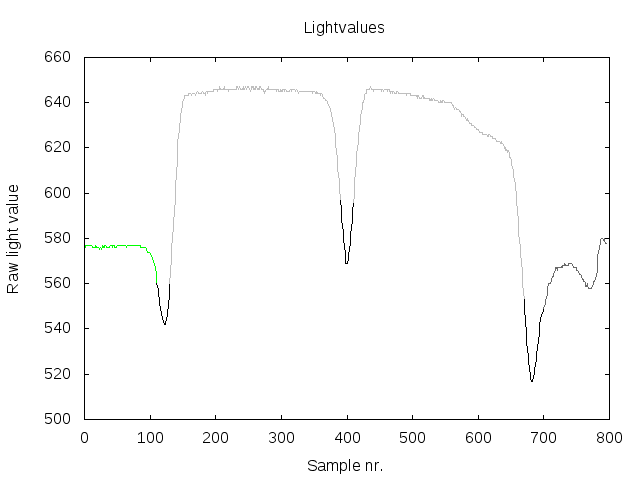
\includegraphics[scale=0.5]{../experiments/1prototype/results/gnuplot/GridAccuracy3cm_color.png}\\
We
tested the light sensors ability to distinguish colors by letting it
start in the green starting zone, drive out across the white area,
crossing a single black line, more white, and finally into the gray
storage area. As seen, green is about the same value as black, which
might cause trouble later on if we need to determine which area we're
in. One solution would be to replace it with a color sensor, but we'll
return to this if it becomes necessary.

\subsection{Conclusion}

We decided on lifting solar panels and storing defect ones in addition
to the line follower. This will make the foundation for our first
prototype, and now we need to start building and testing. However, we
immediately ran into trouble when we started testing the precision of
the line follower. We will continue the testing next time, and depending
on the result, we may change strategies.
